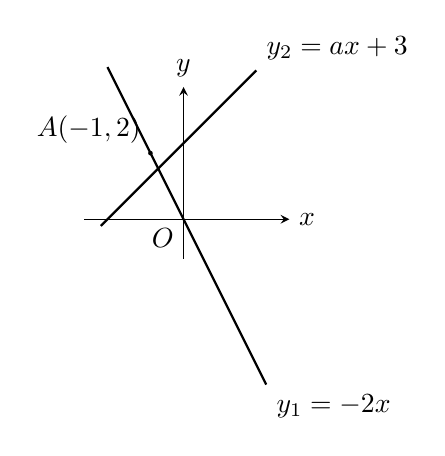
\begin{tikzpicture}[scale=0.42,>=stealth]
  \draw[->] (-3,0)--(3.2,0) node[right] {$x$};
  \draw[->] (0,-1.2)--(0,4) node[above] {$y$};
  \draw[thick] (-2.3,4.6)--(2.5,-5) node[below right] {$y_1=-2x$};
  \draw[thick] (-2.5,-0.2)--(2.2,4.5) node[above right] {$y_2=ax+3$};
  \fill (-1,2) circle (2pt) node[above left] {$A(-1,2)$};
  \node[below left] at (0,0) {$O$};
\end{tikzpicture}
